\chapter{Machine learning}
%\section{What is machine learning?}
\lettrine[lines=3, lhang=0.25, nindent=0em]{\color{Maroon}T}{he Scientific Revolution}
during the Renaissance 
was fuelled by the realisation that Nature can be parametrised using only a handful of equations.
\marginpar{A historical note}
With these tools and sufficient measurements, natural philosophers could use the universal equations to fully model the mechanical universe.
As mathematical tools improved, increasingly more complex systems could be analysed, such as orbits of astrophysical objects or complex optical designs.
Furthermore, the later development of computers allowed for an explosion in the size and breadth of tractable problems, such as dynamics of atomic nuclei, or weather forecast.
%\todo{Compare with Greek/Arabic knowledge}

These applications were either developed from first principles or as effective theories; but contained at their core, relatively simple mathematical models.
For example, the dynamics of $n$-bodies gravitationally interacting are very complicated to solve, but it all spawn from two simple equations, Newton's second law of motion for an object of mass $m$: $\vec{F} = m \cdot \vec{a}$ and the force of gravity between two masses $m_1$ and $m_2$: $F_g=G\frac{m_1  m_2}{r^2}$.

The advent of computers
\marginpar{How do computers fit in?}
 not only gave us mathematical muscle, but it also allowed to connect them to sensors;
providing us with large amounts of data about the real world.
Data that can be used to fit statistical models, even in the absence of underlying mathematical theories, such as recognising objects in images, identifying where in the cell a protein is going to end up, or translating natural language.
The Scientific Revolution of the 16th century brought the concept \emph{``if it can be measured, it can be modelled"}, but the Data Revolution of the 20th century expanded it \emph{``if it can be \emph{represented}, it can be modelled"}.
We went from measuring the variables present in our equations to represent the world in numbers on a computer.

%This opens new oportunities to tackle and explore anything we 

Machine learning \marginpar{Definition of machine learning}
is the study of statistical models that can create inferences from collections of examples. 
In other words, a machine learning model is capable of producing generalised rules from a set of particular cases, an example of induction.
The models can be as concrete as relating the voltage and measured current intensity in a circuit, as complex as relating the sensory input of a rocket with its control, or as abstract as mapping natural images to the text describing its contents.

Instead of designing algorithms that simulate reality from first principles, that can be insurmountably complex and time-consuming; a machine learning model uses data: the algorithm depends on a series of free parameters that are deduced from examples.
\marginpar{The costs}
This flexibility comes with a price: the programmer has relinquished the control to the dataset, and sacrificed the possibility of a mechanistic interpretation.
More on this in Section~\ref{sec:wrong}.

\section{Classification and typology}
Machine learning tasks can be classified according to several criteria.
Here are, in broad strokes, some of the main types that cover the majority of the machine learning problems according to different criteria.

\subsection{Do we have labels?}
\begin{itemize}
\item \emph{Unsupervised:} we do not have data with annotated target values. \emph{Ex: clustering of \DNA{} sequences, dimensionality reduction.}
\item \emph{Supervised:} our training data has assigned labels, and we want to predict them to new data. \emph{Ex: protein secondary structure prediction, linear regression.}
\end{itemize}

The focus of this thesis will be on supervised tasks.

\subsection[Categorical or continuous?]{Are they categorical or continuous?}
The supervised tasks can be again divided depending on the nature of the labels:
\begin{itemize}
\item \emph{Classification:} our labels are categorical variables. \emph{Ex: image recognition, automated transcription of speech, presence or absence of tumours, protein subcellular localisation.}
\item \emph{Regression:} we are interested in the value of continuous variables. \emph{Ex: curve fitting, counting.}
\end{itemize}

\section{The machine learning spectrum}
We can design machine learning models with different degrees of restrictions, or parametric assumptions.
A more restricted model needs less data to converge, and its performance will not be hindered if the underlying assumptions are correct.
On the other hand, if these restrictions are not accurate, the model will be biased and its performance, limited.

If we instead relax the parametric assumptions we obtain a more flexible model, capable of tackling more complex problems.
But this versatility comes with a cost: they require more data to train.

Can we take it to the extreme?
\marginpar{A theoretical result} 
Can we train a model completely free  of assumptions in the case of infinite data? The No Free Lunch Theorem \citep{no_free_lunch} says, averaging over all problems, all algorithms are equally good.
In other words, without inputting domain knowledge that restricts the space of possibilities, we cannot do better than random.
For a given training dataset, an infinite number of models can fit it equally well, while giving completely different answers for any point outside of that.
Domain knowledge can provide us with constraints -- for example, certain physical models must be continuous -- and give us a measure of simplicity -- all else being equal, Ockam's razor would point at the simplest one.

\section{Training and test sets}
To train a supervised model, we need a set of labelled examples, called the \emph{training set},
and a separate and independent set -- the test set -- to evaluate its performance.
\marginpar{The motivation for separated datasets}
Why do we need a separate test set?
It is easy to come up with rules that are perfectly accurate on the training set, but do not generalise well, a phenomenon called \emph{overfitting}.
When presented with a collection of models, we will prefer the ones that have the best performance on the test set.

\section{Evaluating predictions: figures of merit}
How can we compare them?
Figures of merit allow us to evaluate how well the model performs.
Here I will describe some of the most commonly used:

\subsection{Classification problems}
The most obvious measure is the \emph{accuracy}, or the proportion of predictions that are correct.
This is easy to implement and interpret, but it is of limited use on unbalanced datasets: when the number of positive and negative classes are very different.
\marginpar{The problem with unbalance}
For example, if 99\% of our data are negative examples, a model that always predicts the negative class has an accuracy of 99 \%, but it is useless in practice.

In order to get \marginpar{Precision and recall} a more nuanced view we should consider the \emph{precision} -- the fraction of correctly predicted positive examples -- and \emph{recall} -- the fraction of positive examples correctly identified.
A combination \marginpar{$F_1$ score} of both is the $F_1$ score: the harmonic mean of precision and recall:

\begin{equation*}
F_1 = \frac{2}{\frac{1}{precision} + \frac{1}{recall}}
\end{equation*}

\subsection{Regression problems}
When predicting a continuous variable, the simplest measure is the Mean Squared Error, or \MSE.
Often, we want the measure to be in the same units as the input, so we take the square root.
We may also be interested in the correlation between predicted -- $p$ -- and true -- $t$ -- which can be \marginpar{Correlations} expressed by the Pearson correlation R:

\begin{equation*}
R = \frac{\sum_{i=1}^N (p_i - \bar{p}) (t_i - \bar t)}{\sqrt{\sum_{i=1}^N (p_i - \bar{p})^2} \sqrt{\sum_{i=1}^N(t_i - \bar t)^2}}
\end{equation*}

This measures the linear correlation between two variables, and can be affected by outliers. \marginpar{Spearman}
An alternative is the Spearman correlation, which computes the Pearson R on the indexes.

\section[Traditional machine learning]{A point of comparison: traditional machine learning}
In this section, I will give an overview of some of the most popular supervised machine learning algorithms to illustrate how they work, and the type of underlying assumptions they operate under.
I will describe them in their simplest form, be it for regression or classification, but both can be easily generalised: a regression algorithm can be turned to a binary classifier mapping the positive and negative labels to $(1, -1)$ or vice-versa.
A binary classifier can be used in a problem with $N$ classes by either training $N$ binary classifiers for each class versus the rest, or all the $\binom{N}{2}$ pairwise binary classifications.

\subsection[Linear regression]{Linear regression: Ordinary Least Squares, Ridge, and \LASSO}\label{sec:linear}
Ordinary Least Squares (\OLS) is the simplest linear regression model: the linear combination of the inputs that minimises the squared error.
For a matrix $ \widetilde X$ of observations and a vector of target $\vec y$, \OLS{} finds the vector $\vec w = (w_0, w_1, ... w_d)$ that minimises the loss:

\begin{equation*}
 L_{\OLS} = || \widetilde  X \vec w - \vec y ||_2 ^2,
\end{equation*}
where $d$ is the number of dimensions of the inputs, ie., the number of input features.

This method is simple and can be solved efficiently by linear algebra libraries through, for example, an \textsc{lu}{} decomposition\footnote{A standard procedure to solve systems of equations, where the matrix $\widetilde{X}$ is factored into the product of a lower and an upper triangular matrices, without needing to explicitly invert the matrix. Then, the components of $\vec w$ can be obtained iteratively.}.
But if there is co-linearity between input features, the matrix $ \widetilde X$ is close to singular, so its inverse can become numerically unstable.

A simple solution \marginpar{Ridge} is to add a term that tends to shrink the coefficients of $\vec w$, and makes the solution unique even in the singular case:

\[ L_{Ridge} = || \widetilde  X \vec w - \vec y ||_2 ^2 + \lambda ||\vec w||_2^2,\]
where $\lambda$ regulates the strength of this shrinkage.
Since the penalisation depends on the $L^2$ norm of the vector $w$, the weight of co-linear features will be ``distributed" amongst them.

Sometimes, we want sparse weights, \marginpar{\LASSO} for example, if we know some features are irrelevant, but we do not know which ones.
We can then use $L^1$ regularisation:

\[ L_{\LASSO} = || \widetilde X \vec w - \vec y ||_2 ^2 + \alpha ||\vec w||_1^2,\]
where $\alpha$ is our new regularisation strength parameter.
The higher it is, the more weights will be close to $0$.

%LASSO cannot be solved analytically, so we need to use iterative methods.
This is a good point to introduce
\marginpar{Parameters and hyperparameters}
some important vocabulary in machine learning:

\begin{itemize}
	\item \emph{Parameters} are a set of numbers involved in the algorithm inferred from the data.
	In this case, the components of the vector $\vec{w}$ are the parameters learned.
	\item {Hyperparameters} are the settings decided on by the human.
	In this case, the strength of the regularisations, $\alpha$ and $\lambda$, are hyperparameters, but also the decision to use one or the other.
\end{itemize}
 
\subsection{Logistic regression}\label{sec:logistic_regression}
Logistic regression \marginpar{Linear models for classification} is an adaptation of linear models for classification.
The output of the linear model is wrapped by a logistic function:

\begin{equation*}
f(\vec x) = \frac{1}{1 + e^{- \vec{w} \cdot \vec x}}
\end{equation*}

It can also be generalised to $N$ multiple mutually exclusive classes.
Each class has one linear model given by the vector of weights $\left\{\vec w_i \right\}_{i=1} ^N$:

\begin{equation*}
\begin{bmatrix}z_1 \\ z_2 \\ \vdots \\ z_N\end{bmatrix} = 
\begin{bmatrix}
\vec w_1 \vec{x} \\ \vec w_2 \vec{x} \\ \vdots \\ \vec w_N \vec{x}
\end{bmatrix} = 
\widetilde W \cdot \vec{x},
\end{equation*}
where $\widetilde W$ is an $(N \times d)$ matrix.
The components of the vector $\vec{z}$ are called the \emph{logits}. 
To obtain probabilities we use the exponential to make them all positive and normalise the sum.
\marginpar{Softmax}
This is called the softmax function:

\begin{equation*}
\sigma(\vec{z})_i = \frac{e^{z_i}}{\sum_j^N e^{z_j}}
\end{equation*}

If the logits are scaled up, the softmax will be more concentrated around the maximum, suggesting a more confident prediction.
As before, we can apply $L^1$ or $L^2$ regularisations, which imply lower coefficients on $W$, ergo lower values for the logits.
A stronger regularisation returns a less confident predictor, as shown in Figure~\ref{fig:logistic}.
In particular, \ref{subfig:logistic_strong}, has a much narrower region of uncertain predictions. 

\begin{figure}
	\centering
	\subcaptionbox{Weak regularisation}{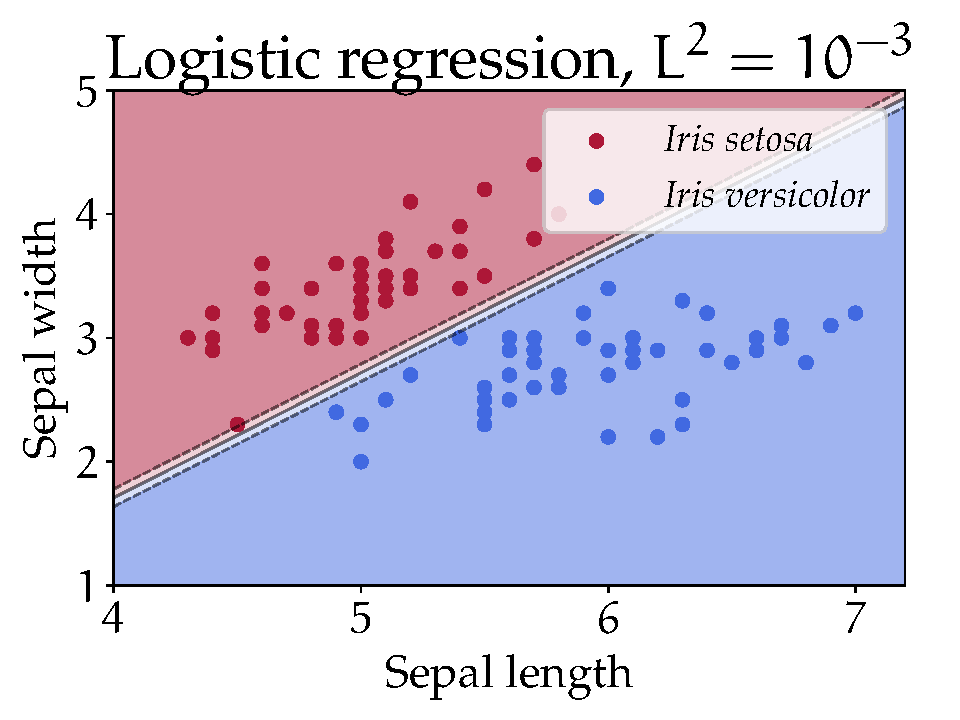
\includegraphics[width=0.45\textwidth]{machine_learning/figures/logistic_3}}
	\subcaptionbox{Strong regularisation\label{subfig:logistic_strong}}{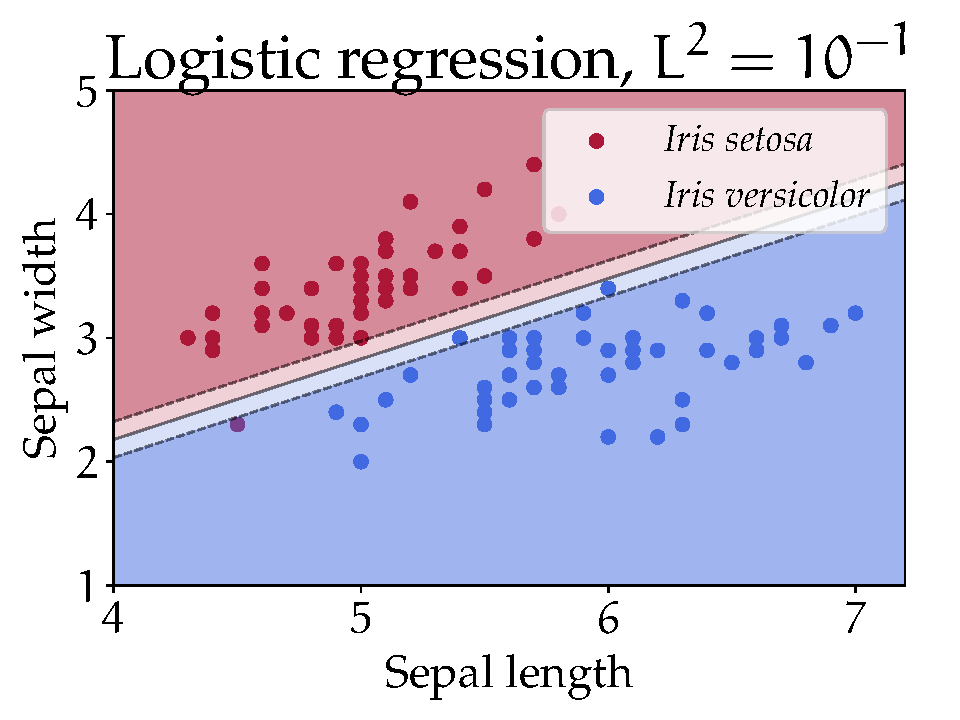
\includegraphics[width=0.45\textwidth]{machine_learning/figures/logistic_1}}
	\caption{Classification of two species of Iris flowers according to the length and width of sepals using logistic regression.}\label{fig:logistic}
\end{figure}


\subsection{Multi-Layer Perceptron}\label{sec:mlp}
A linear model on $d$ features is limited to $d$ free parameters, or at most $d \cdot N$ for $N$ classes, and is limited to linear functions.
When we have more complicated tasks, and more data for them, we would like to be able to learn more parameters.
A simple way to do so is to build upon linear models, and have an intermediate \emph{hidden state} $\vec{h}$ of arbitrary dimension.
The vector of probabilities for every class is then:

\begin{align*}
\vec{h} &= \widetilde W_1 \cdot \vec{x} \\
\vec{z} &= \widetilde W_2 \cdot \vec{h} \\
p(\vec x \in i) &= \sigma(\vec z)_i
\end{align*}
where the last line is only necessary for classification.

Although we now have more free parameters -- the components of the matrices $W_1$ and $W_2$ -- the model is exactly equivalent to a linear model, since the two matrices $W_1$ and $W_2$ act right one after the other, so can be multiplied together to recover our equivalent weights.
This can be fixed by introducing an arbitrary non-linear function $f$ to the hidden layer:

\begin{align*}
\vec{h} &= \widetilde W_1 \cdot \vec{x} \\
\vec{z} &= \widetilde W_2 \cdot f(\vec{h}) \\
p(\vec x \in i) &= \sigma(\vec z)_i
\end{align*}

Since we have no constraints over the properties of $f$, common choices are simple point-wise functions, such as $\tanh(x)$; the logistic, $\frac{1}{1 + e^{-x}}$; or the Rectified Linear Unit, $ReLU(x)=[x \; if \; x > 0 \; else \; 0]$.

We can repeat the same procedure and chain two hidden layers:

\marginpar{More layers!}
\begin{align*}
\vec{h_1} &= \widetilde W_1 \cdot \vec{x} \\
\vec{h_2} &= \widetilde W_2 \cdot f(\vec{h_1}) \\
\vec{z} &= \widetilde W_3 \cdot f(\vec{h_2}) \\
p(\vec x \in i) &= \sigma(\vec z)_i
\end{align*}

The training is done by computing the gradients of the loss -- the measure of how wrong our predictions are -- with respect to every parameter -- the matrix elements -- given a set of data, and updating the weights accordingly.
We will discuss this in more detail in Section~\ref{sec:grad_descent}.
While there is no theoretical limit to how many hidden layers can be added, but two is the practical limit.
This is because adding layers degrades the gradient from the previous ones, making it harder to converge, as the information cannot reach the first layers.


\subsection{Support Vector Machines}
A Support Vector Machine, or \SVM, is in its simplest form, a supervised, binary classification algorithm that tries to find the hyperplane that maximises the separation of the two groups.
To account for noise, a slack parameter, that will ignore points that are too close to the boundary can be included.
Figure~\ref{fig:svm} illustrates an example of classifying two species from the classic Iris dataset~\citep{iris_dataset}.


\begin{figure}
\centering
\subcaptionbox{Linear kernel}{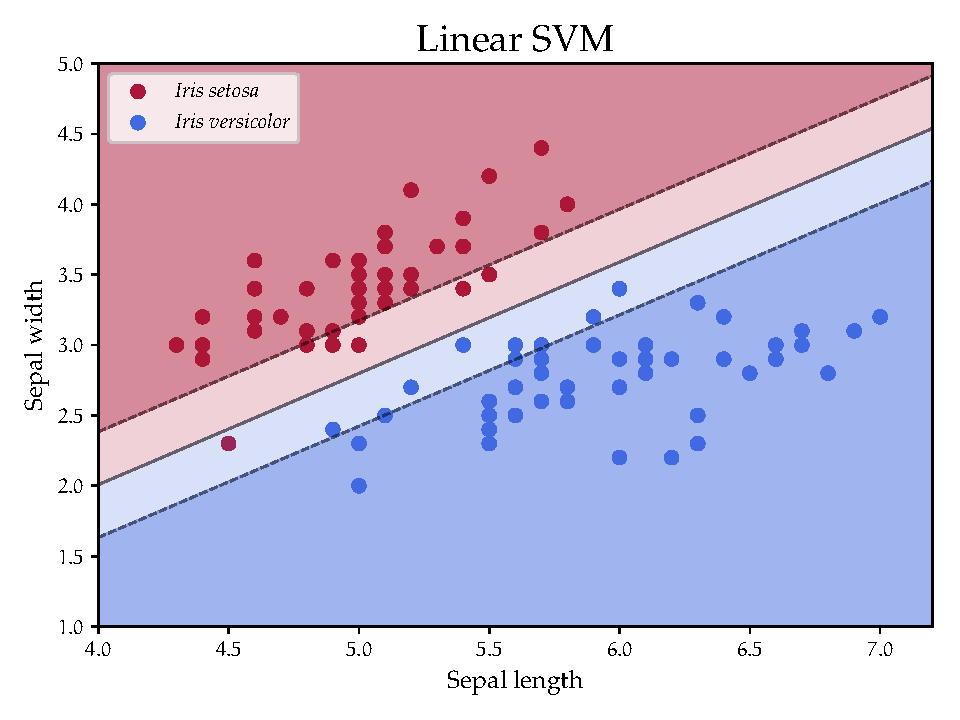
\includegraphics[width=0.45\textwidth]{machine_learning/figures/svm.pdf}}%
\hfill
\subcaptionbox{\RBF{} kernel\label{subfig:svm_rbf}}{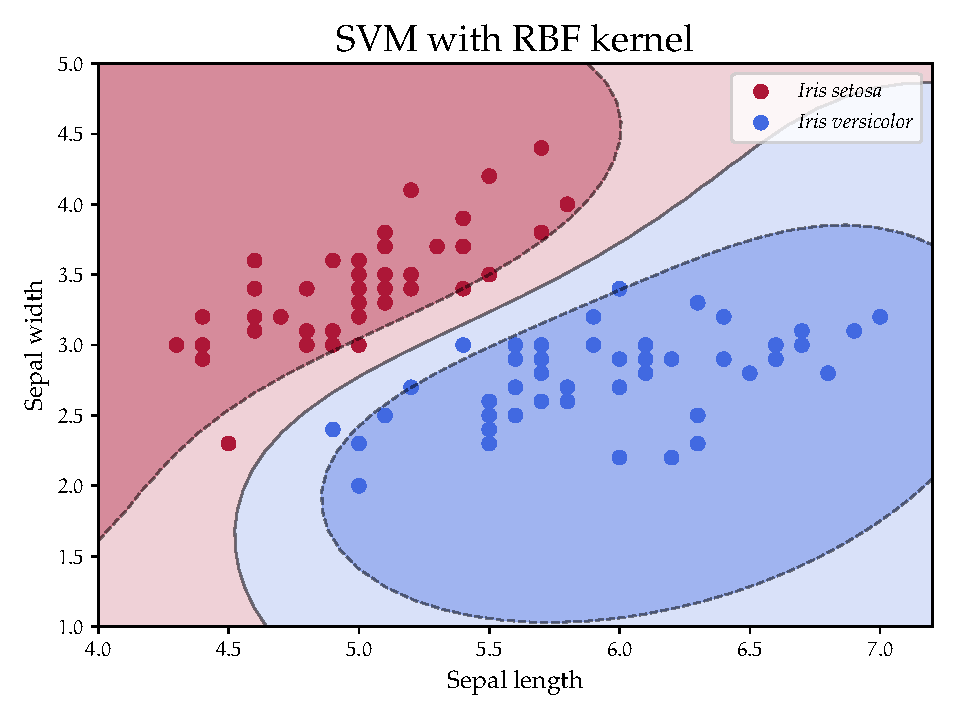
\includegraphics[width=0.45\textwidth]{machine_learning/figures/svm_rbf.pdf}}%
\caption{Classification of two species of Iris flowers according to the length and width of sepals using Suport Vector Machines.}\label{fig:svm}
\end{figure}

It can be generalised \marginpar{The kernel trick} to non-flat boundaries using the so-called \emph{kernel trick}, where Euclidean distances are replaced with an arbitrary measure of similarity given by positive-definite kernel function:
\[||\vec{x}_1 - \vec{x}_2|| \rightarrow k(\vec{x}_1, \vec{x}_2)\]

For example, in Figure~\ref{subfig:svm_rbf} we have used a Radial Basis Function:

\[k(\vec{x}_1, \vec{x}_2) = e^{-\gamma ||\vec{x}_1 - \vec{x}_2||^2 },\]
which implicitly projects the data into an infinite-dimensional space.

Another way of interpreting the kernel trick is to think of it as learning a topological transformation of the space that makes the data separable by the final hyperplane, a linear function.

\subsection{\emph{k}-Nearest Neighbour}
The Nearest Neighbour classifier takes the $k$ closest points in the training set and predicts the most common label.
\marginpar{Bias-variance tradeoff}
The choice of $k$ is a balance between noise and flexibility: smaller values give more distinct frontiers but are more susceptible to noise.

\begin{figure}[htb]
	\centering
	\subcaptionbox{Closest neighbour ($k=1$)}{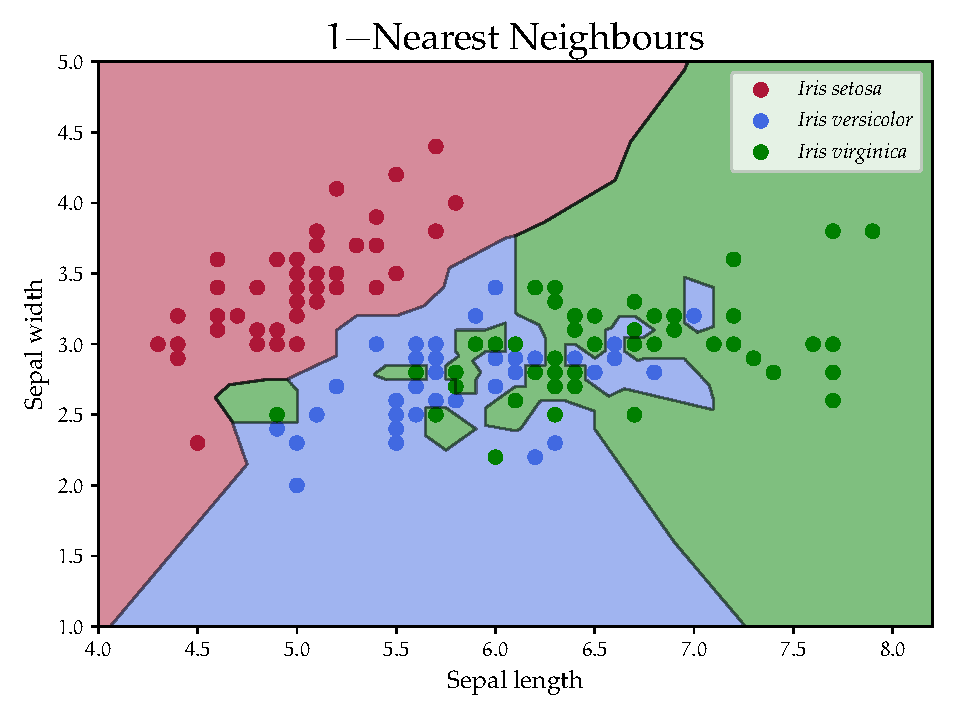
\includegraphics[width=0.45\textwidth]{machine_learning/figures/knn_1}}
	\hfill
	\subcaptionbox{Average of the five closest neighbours. ($k=5$)}{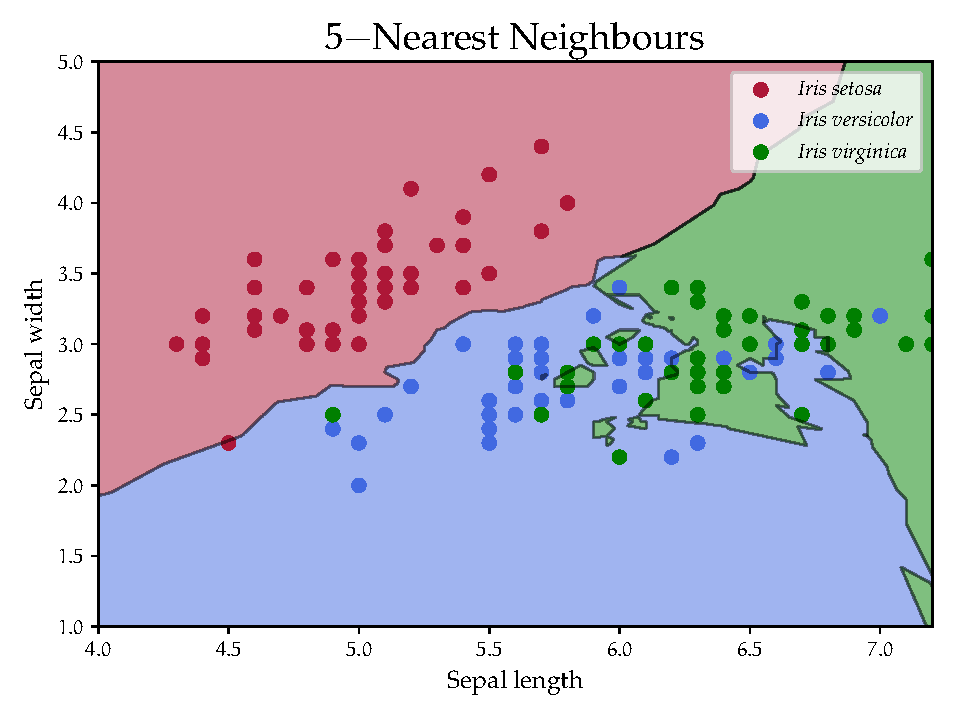
\includegraphics[width=0.45\textwidth]{machine_learning/figures/knn_5}}
	\caption{Classification of three species of Iris flowers according to the length and width of sepals using Nearest Neighbour.}\label{fig:knn}
\end{figure}

\subsection{Decision tree}\label{sec:decision_tree}
Decision trees are based on a measure of impurity of a sample: the more homogeneous, the less impure it is.
The most common is the Gini impurity:

\[ G(\vec x) = \sum_k p_{k} (1-p_k),\]
where $p_k$ is the fraction of labels equal to $k$ in the group.

A decision tree splits recursively the training based on the feature that gives the highest decrease in Gini impurity, as illustrated in Figure~\ref{subfig:gini}.
The final result is a series of simple boolean rules that can be interpreted by humans.
Figure~\ref{subfig:tree_explained} is an example: the root of the tree -- shown in white -- contains all the training points, and each branch splits it according to a single feature.
The process is repeated until no more cuts can improve the performance, or until the tree reaches a maximum depth.

\begin{figure}[tb]
	\subcaptionbox{Gini impurity as a function of the first split.
	The ideal cut is selected.\label{subfig:gini}}{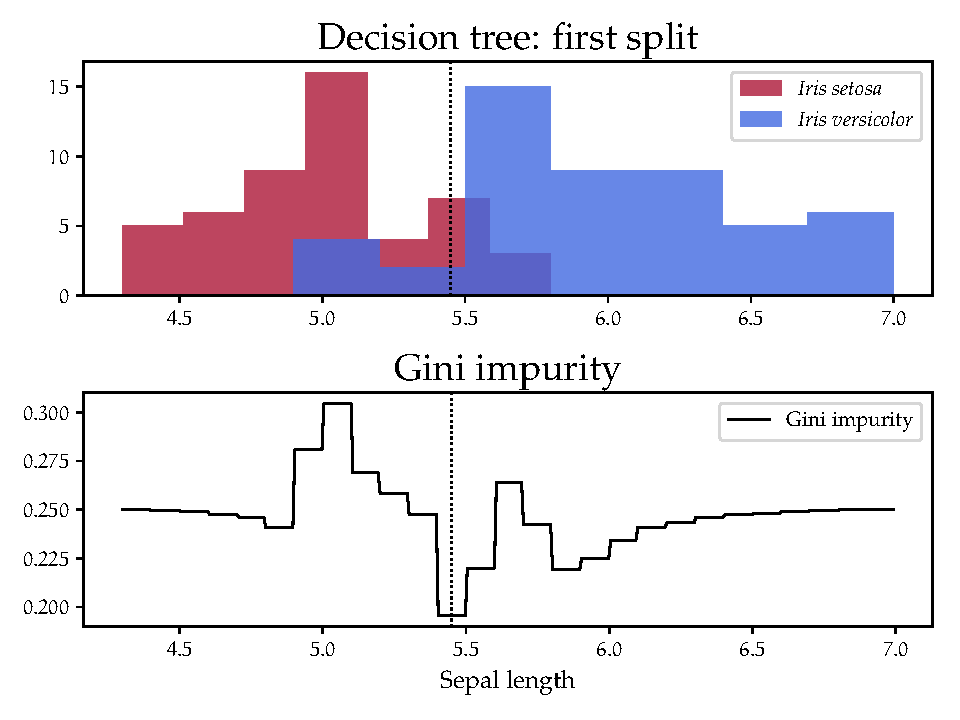
\includegraphics[width=0.45\textwidth]{machine_learning/figures/tree_split}}
	\hfill
	\subcaptionbox{Regions predicted by the tree.\label{subfig:tree}}{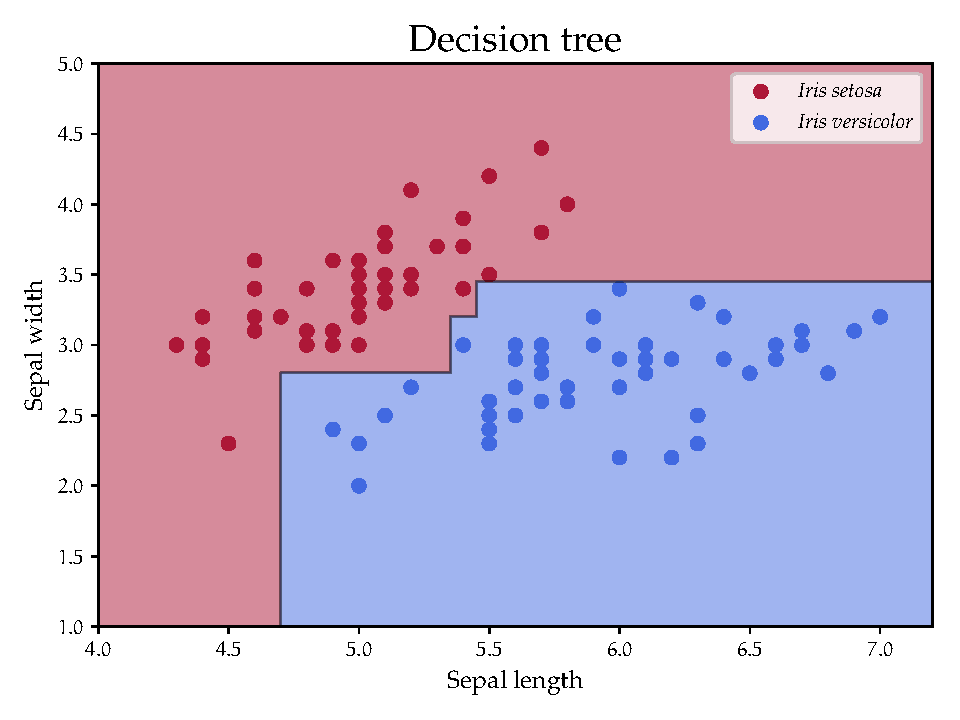
\includegraphics[width=0.45\textwidth]{machine_learning/figures/tree_2d}}
	\caption{Classifications made by a decision tree on the Iris species dataset.}\label{fig:tree}
\end{figure}

\newgeometry{outer=10mm, inner=10mm}
\begin{figure}[tb] %[p]age of floats
	\centering
	%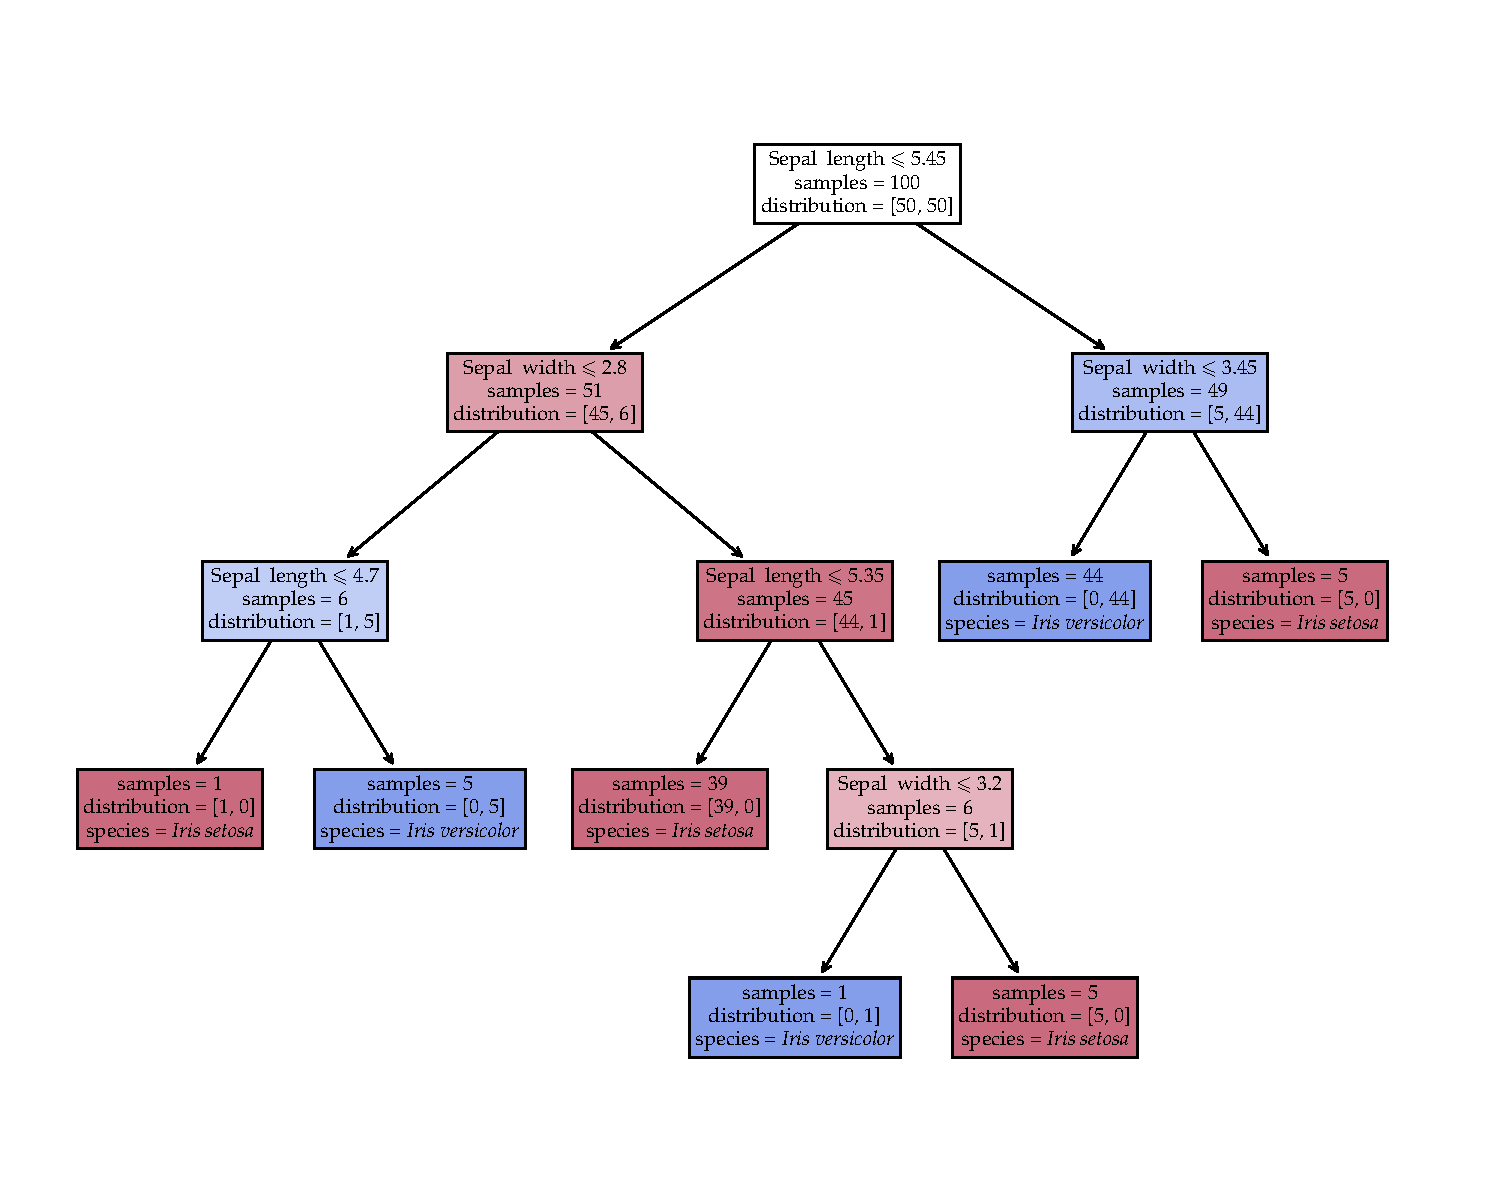
\includegraphics[width=1.2\textwidth]{machine_learning/figures/tree}
	%\makebox[\paperwidth][l]{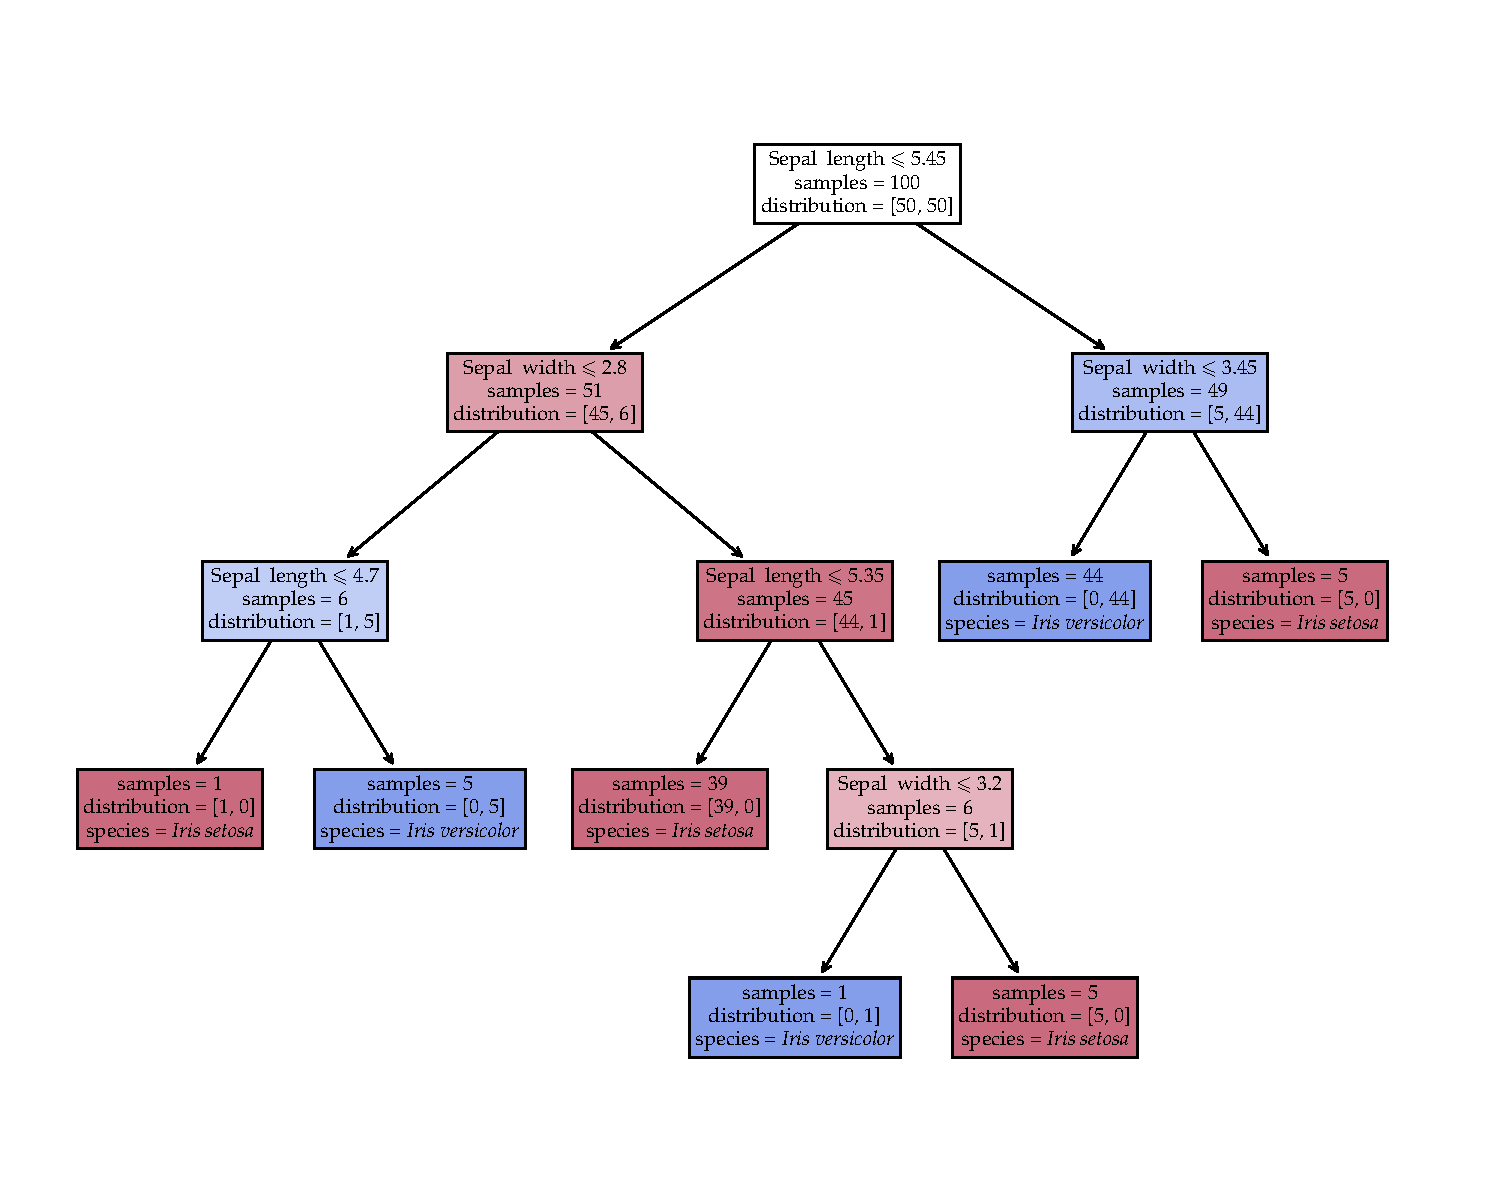
\includegraphics[width=1.2\textwidth]{machine_learning/figures/tree}}
	%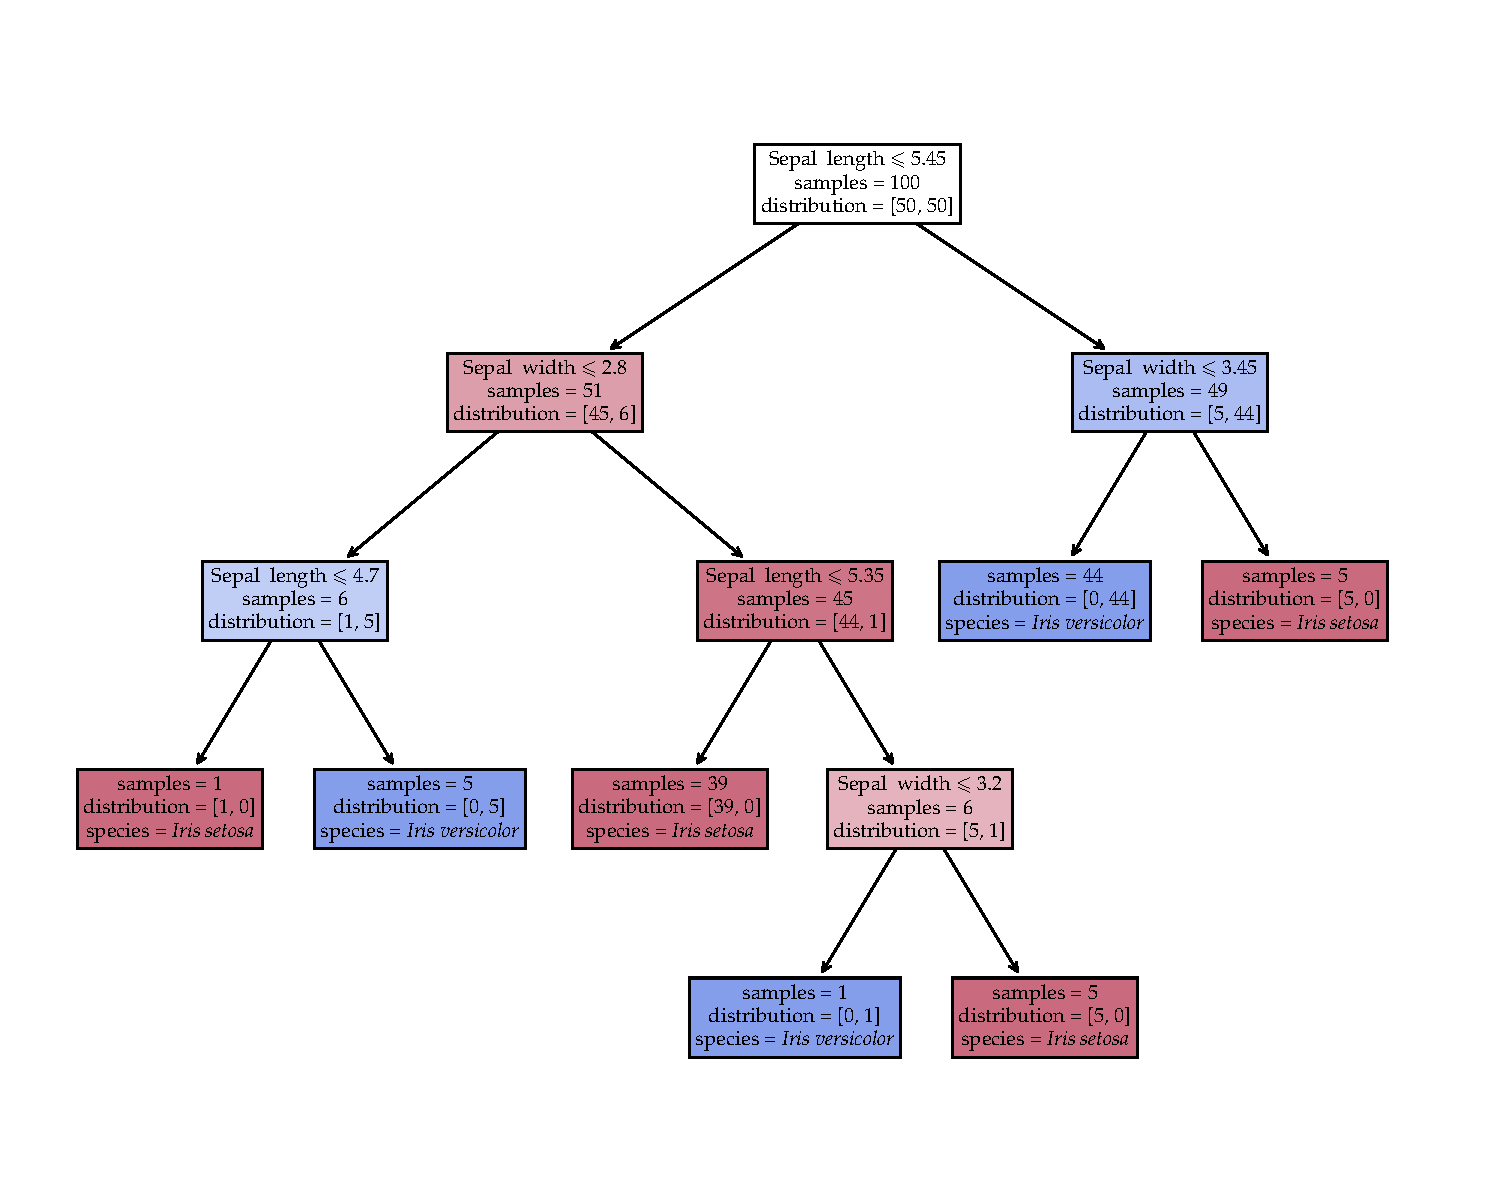
\includegraphics[width=1.2\textwidth, center]{machine_learning/figures/tree}
	%\fcolorbox{black}{red}{
	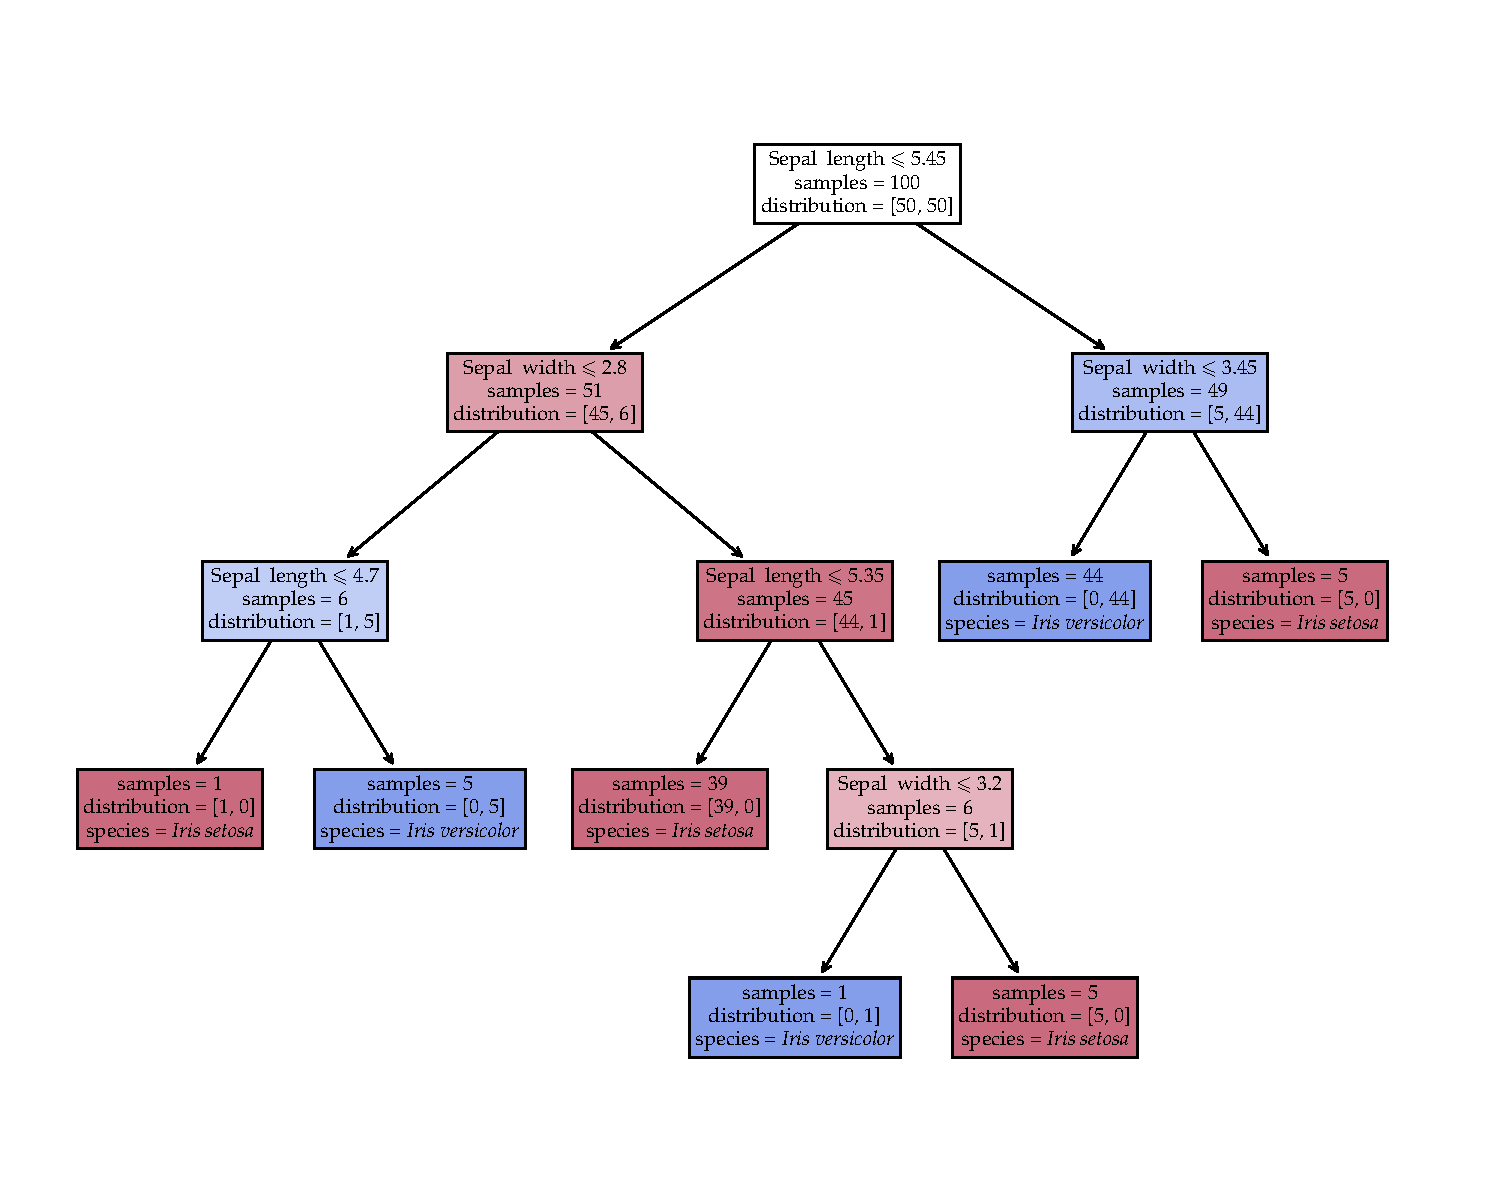
\includegraphics[trim={24mm, 33mm, 5mm, 14mm}, clip, width=1.\textwidth]{machine_learning/figures/tree}
	%}
	\restoregeometry
	\caption{The rules of a decision tree are interpretable.
	The saturation of the background corresponds to the purity of the node.
	While a human can read them, they do not make much sense to us,
	it is just splitting the space, one feature at a time.\label{subfig:tree_explained}}
\end{figure}
\restoregeometry

\subsection{Random Forest}\label{sec:random_forest}
A Random Forest is an ensemble of decision trees, as described in Section~\ref{sec:decision_tree}.
Each tree is trained on a random subset of the data, and the final score is a vote across the trees.
Furthermore, for every split, we only consider a new random subset of the features, to increase diversity.
The advantage over a single decision tree is that now we have an ensemble of trees, each trained on slightly different data.
\marginpar{Bias-variance tradeoff}
Since every data point is only considered by a fraction of the trees, the random forest is more robust against noise; but for the same reason, it will not be able to model so well outliers.


\subsection{Gaussian Processes}
A Gaussian Process (\GP) takes as an input a set of data points $(x, y)$ that are assumed to be generated by a latent, unknown function $f(x)$ that we wish to infer, plus Gaussian noise. The output is a \emph{probability distribution} over functions, that should be interpreted as the likelihood for each given function to have produced the observed data.


\begin{figure}[htb]
	\centering
	\subcaptionbox{Complete data}{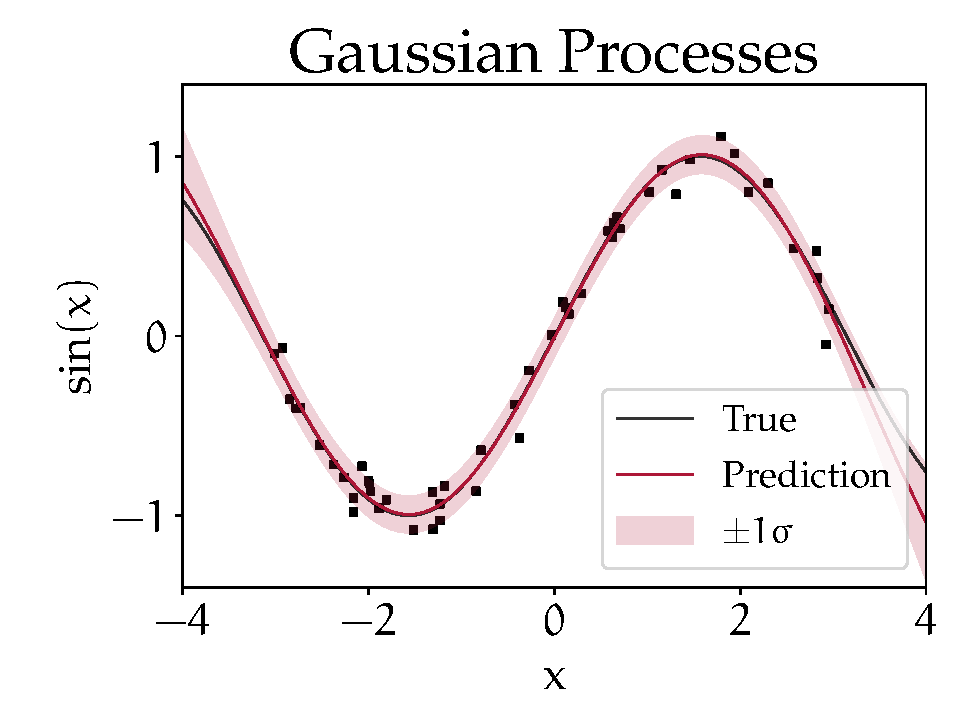
\includegraphics[width=0.45\textwidth]{machine_learning/figures/sin_toy}}
	\hfill
	\subcaptionbox{Gapped data.}{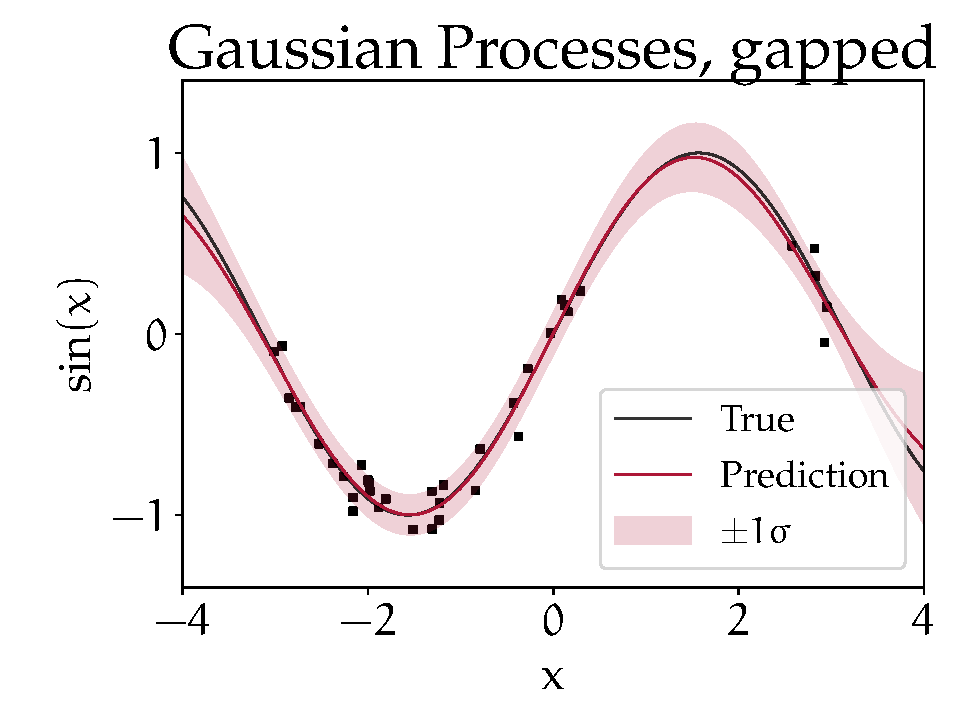
\includegraphics[width=0.45\textwidth]{machine_learning/figures/sin_toy_gapped}}
	\caption{Reconstruction of the $\sin$ function using Gaussian Processes.
	Note the larger uncertainty when there is a gap in the training set.}\label{fig:gp_toy}
\end{figure}


Consider a vector space over functions\footnote{This is a mathematical justification. If you are not interested in Hilbert spaces, jump to the last equation.}, called Hilbert space $\mathscr{H}$, and define a complete, orthonormal basis $\{\phi_i(x)\}_{i=0}^{n}$.
Any function $f$ in this space can be decomposed as a linear combination of the basis:

 \[f(x) = \sum_{i=0}^{n} c_i \phi_i(x)\]
 
In GP, we define our Hilbert space through a positive semi-definite \emph{covariance function} $k(x, x')$.
This induces a metric defined through the distance:

	\[	d(f, g) =\int_{\mathcal{R}}  f(x) k(x, x') g(x') dx dx', \]
and a series of eigenfunctions of the covariance function.
	
For example,\marginpar{\RBF{} appears again} the previously seen radial basis covariance function defines the Hilbert space of $C^\infty \cap L^2$ functions: all the smooth functions of square-integrable..
	
The GP will thus project our $n$ data points into this $N$-dimensional space -- in general, $N >> n$; usually $N = \infty$. Note that, due to geometry, our $n$ data points must live in an $n$-dimensional subspace of $\mathscr{H}$.
The output is an estimation $\hat f$ of our latent function $f$, that can be interpreted as a decomposition in the eigenfunctions of our covariance function.
	
	\[\hat f(x) = \sum_{i=0}^{n} c_i \phi_i(x)\]
	
But, unlike other procedures, $c_i$ have probability distributions over them.
We can use them to sample likely candidates for the latent function, as shown in Figure~\ref{fig:gp_sampling}.
	
\begin{figure}[hbt]
\centering
	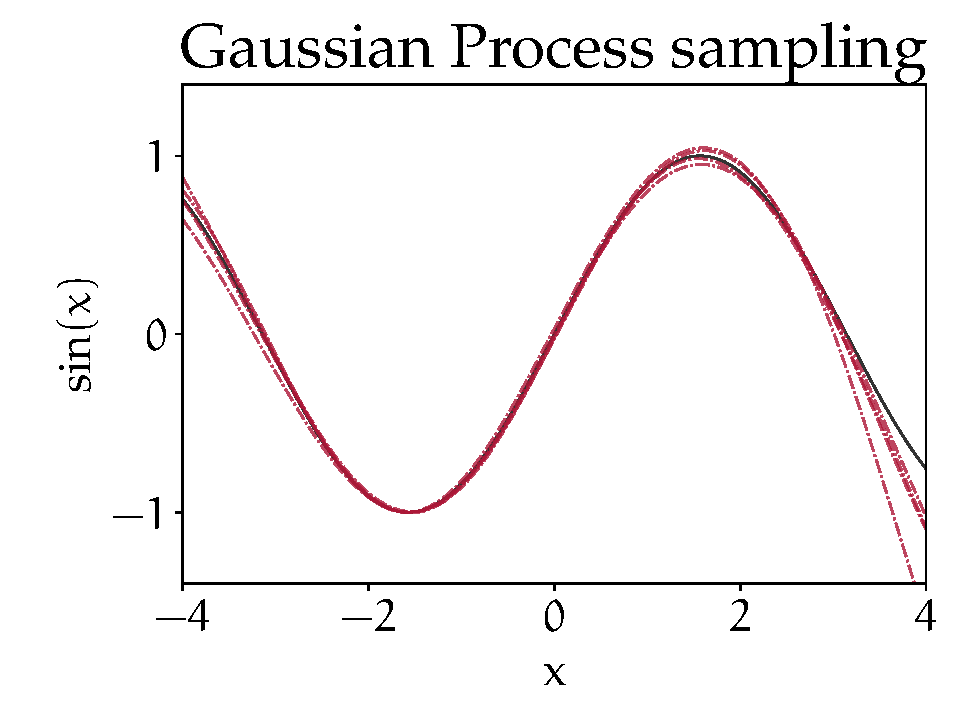
\includegraphics[width=0.7\textwidth]{machine_learning/figures/sin_samples}
	\caption{Posterior samples from Gaussian Processes.}\label{fig:gp_sampling}
\end{figure}

\subsection{Isotonic regression}
Isotonic regression minimises the squared errors of a function that is piecewise constant, and non-decreasing.
Given enough data points, it can fit arbitrarily complex curves, as long as they are monotonous.
This method is particularly useful in calibration to turn predicted scores into actual probabilities.

\begin{figure}[hbt]
	\centering
	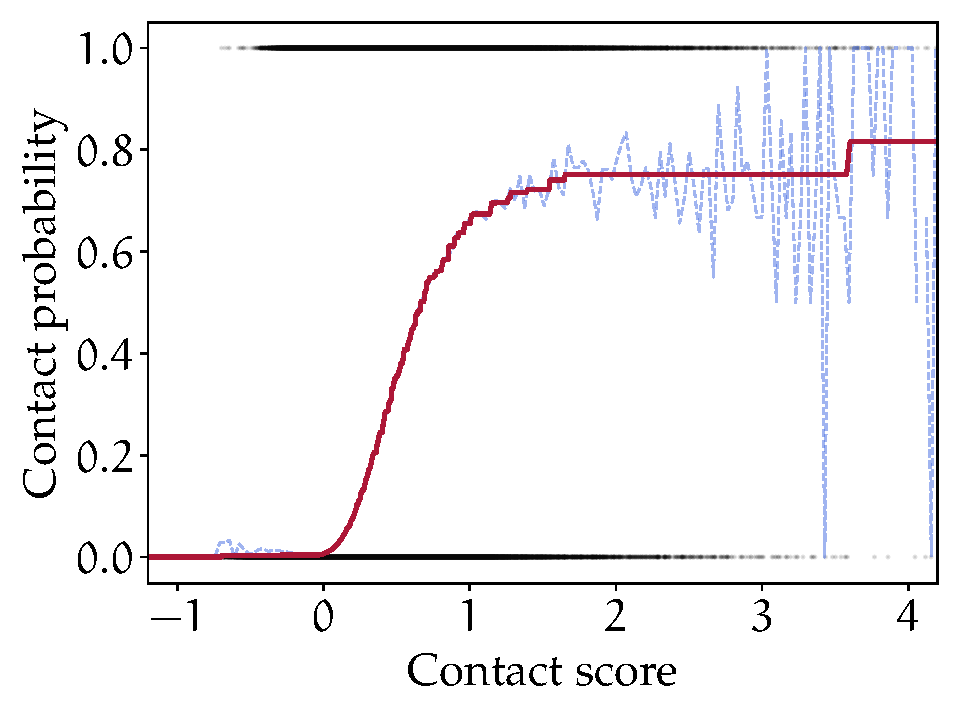
\includegraphics[width=0.7\textwidth]{machine_learning/figures/isotonic}
	\caption{Example of Isotonic regression applied for calibration.
	On the x-axis is the score given by \GaussDCA, a statistical method that correlates with the probability of two residues being in contact (more information on Section~\ref{sec:contacts}).
	The black dots are the data points, the dotted line is a simple binning, and the solid line is the isotonic regression.
	The isotonic regressor does not require to define a number of bins up front which would make it susceptible to noise in too small bins.}\label{fig:isotonic}
\end{figure}



\section{On the wrongness of machine learning}\label{sec:wrong}
The results of machine learning can be impressive and may lead to think too much of them.
But in their power lies their weakness: they can blindly extract a signal from the training data without humans needing to guide it, but that means they are incapable of reasoning.
Since they lack a mechanistic model, they can find correlations, but not causations.

Furthermore, they are vulnerable to outliers.
Training a machine learning model means finding the set of parameters that ``best" fit the training points, but we have no constraints outside of that.
If we were to feed it input data that are sufficiently far away from what was used to train, our outputs will be, essentially, unconstrained.
A machine learning model is a mathematical function, which means it will always give us an answer, but in general, and unlike a human, it lacks the capability of murmuring \emph{``that is strange..."}.

In general, a machine learning model can only get to be as good as the data it was used to train it, and will always incorporate all of its biases and limitations.

